%%%%%%%%%%%%%%%%%%%%%%%%%%%%%%%%%%%%%%%%%%%%%%%%%%%%%%%%%%%%%%%%%%%%%%%%%%
% Copyright (c) 2013, ETH Zurich.
% All rights reserved.
%
% This file is distributed under the terms in the attached LICENSE file.
% If you do not find this file, copies can be found by writing to:
% ETH Zurich D-INFK, Universitaetstr. 6, CH-8092 Zurich. Attn: Systems Group.
%%%%%%%%%%%%%%%%%%%%%%%%%%%%%%%%%%%%%%%%%%%%%%%%%%%%%%%%%%%%%%%%%%%%%%%%%%

\documentclass[a4paper,twoside]{report} % for a report (default)

\usepackage{bftn} % You need this
\usepackage{multirow}
\usepackage{listings}
\usepackage{color}

\title{Barrelfish on ARMv7}   % title of report
\author{Simon Gerber \and Stefan Kaestle \and Timothy Roscoe \and
  Pravin Shinde \and Gerd Zellweger}
\tnnumber{017}  % give the number of the tech report
\tnkey{ARMv7} % Short title, will appear in footer

% \date{Month Year} % Not needed - will be taken from version history

\newcommand{\todo}[1]{\note{\textbf{TODO:} #1}}

\begin{document}
\maketitle

\newcommand{\code}[1]{{\lstinline!#1!}}
\newcommand{\file}[1]{{\lstinline!#1!}}

%configure listings properly
\lstset{%
  basicstyle=\small\ttfamily,
  escapechar=@
}

\newcommand{\shell}{\$}
\newcommand{\home}{\$HOME}

\newcommand{\stefan}[1]{%
  {\color{red}[{\color{red}{SK}} #1]}}

\newcommand{\gerd}[1]{%
  {\color{red}[{\color{red}{GZ}} #1]}}

\newcommand{\simon}[1]{%
  {\color{red}[{\color{red}{SG}} #1]}}

\newcommand{\pravin}[1]{%
  {\color{red}[{\color{red}{PS}} #1]}}


%
% Include version history first
%
\begin{versionhistory}
\vhEntry{0.1}{05.12.2013}{SK}{Initial version}
\end{versionhistory}

% \intro{Abstract}		% Insert abstract here
% \intro{Acknowledgements}	% Uncomment (if needed) for acknowledgements
\tableofcontents		% Uncomment (if needed) for final draft
% \listoffigures		% Uncomment (if needed) for final draft
% \listoftables			% Uncomment (if needed) for final draft

\lstset{
  language=C,
  basicstyle=\ttfamily \small,
  flexiblecolumns=false,
  basewidth={0.5em,0.45em},
  boxpos=t,
}

\newcommand{\eclipse}{ECL\textsuperscript{i}PS\textsuperscript{e}\xspace}
\newcommand{\codesize}{\scriptsize}
\newcommand{\note}[1]{[\textcolor{red}{\emph{#1}}]}

%%%%%%%%%%%%%%%%%%%%%%%%%%%%%%%%%%%%%%%%%%%%%%%%%%%%%%%%%%%%%%%%%%%%%%%%
\chapter{Introduction}

This document describes the state of support for ARM processors
in Barrelfish.

ARM hardware is highly diverse, and has evolved over time.  As a
research OS, Barrelfish focusses ARM support on a small number of
platforms based on wide availability, ease of maintenance, and
research interest.  

The principal processors with ARM support in Barrelfish at present are
as follows: 

\begin{itemize}
\item ARMv7a (Cortex A-series), in particular the Cortex A9. 
\item ARMv7m (Cortex M-series), in particular the Cortex M3. 
\item ARMv5 processors, in particular the Intel iXP2800 network
  processor (which uses an XScale core). 
\end{itemize}

The main systems we target at present are:
\begin{itemize}
\item The Texas Instruments OMAP4460 SoC used in the Pandaboard ES
  platform. 
\item The ARM VExpress\_EMM board, under emulation in the GEM5
  simulator. 
\end{itemize}

In addition there is limited (and not tested) support in the
Barrelfish tree for:
\begin{itemize}
\item The Netronome i8000 card, incorporating a single Intel iXP2800
  processor. 
\end{itemize}


%%%%%%%%%%%%%%%%%%%%%%%%%%%%%%%%%%%%%%%%%%%%%%%%%%%%%%%%%%%%%%%%%%%%%%%%
\chapter{General ARM compilation}
\label{sec:armcompile}

We now describe the OMAP4460 and GEM5 Barrelfish implementation issues
and build steps. 

This section assumes a properly set up toolchain for Barrelfish as
described in the latest README file.

Compiling ARM support in Barrelfish requires a cross-compilation
toolchain on the programmers \texttt{PATH}.  For ARMv7 support we use
the MentorGraphics codesourcery toolchain, at time of writing the
release version of 2012.03.  To check that the toolchain is set up
correctly: 
\begin{lstlisting}
@\shell@ arm-linux-gnueabi-gcc --version
arm-linux-gnueabi-gcc (Sourcery CodeBench Lite 2012.03-57) 4.6.3
Copyright (C) 2011 Free Software Foundation, Inc.
This is free software; see the source for copying conditions. There is NO
warranty; not even for MERCHANTABILITY or FITNESS FOR A PARTICULAR PURPOSE.
\end{lstlisting}

%--------------------------------------------------
\chapter{OMAP4460 specifics}

% Source: Claudio 3.1

The OMAP4460 is a system on a chip (SoC) by Texas Instruments,
intended for use in consumer devices like smartphones and tablet
computers. It contains:

\begin{itemize}
\item A dual core ARM Cortex-A9 processor
\item Two ARM Cortex-M3 processors
\item A hardware spinlock module
\item A mailbox module
\item Many devices to process media input and output
\end{itemize}

The intention is that the Cortex-A9 will be running a general purpose
operating system, while the Cortex-M3 processors will only be running
a real-time operating system to control the imaging subsystem.

The processor configuration in the OMAP4460 is somewhat
unconventional; for example, the Cortex-M3 processors share a
custom MMU with page faults handled by code running on the Cortex-A9
processors and hence are constrained to run in the same virtual
address at all times.  They are also not cache-coherent with the
Cortex-A9 cores. 

\section{Compiling and booting}

To compile Barrelfish for the Pandaboard, first configure your
toolchain as described in Section~\ref{sec:armcompile}. Then execute: 

\begin{lstlisting}
cd @\shell@SRC
mkdir build
cd build
../hake/hake.sh -a armv7 -s ../
make pandaboard_image
\end{lstlisting}

The resulting image can be booted on the Pandaboard over the USB OTG
connector using the standard \texttt{usbboot} utility.  It will
generate console output on the Pandaboard's serial connector.

\section{Booting the second OMAP A9 core}

% source: AOS m6

Here is a brief overview of how the bootstrapping process for the second core
works: it waits for a signal from the BSP core (an interrupt), and when this
signal is received, the application core will read an address from a well-
defined register and start executing the code from this address.

To boot the second core, one can write the address of
a function to the register and send the inter-processor
interrupt. Following are some pointers to the documentation to help
understand the bootstrapping process in more detail:

\begin{itemize}
\item Section 27.4.4 in the OMAP44xx manual talks about the boot process for
  application cores.
\item Pages 1144 \textit{ff.} in the OMAP44xx manual have the register
  layout for the registers that are used in the boot process of the
  second core. 
\end{itemize}

Note that the Barrelfish codebase distinguishes between the BSP (bootstrap)
processor and APP (application) processors. This distinction and naming
originates from Intel x86 support where the BIOS will choose a
distinguished BSP processor at start-up and the OS 
is responsible for starting the rest of the processors (the APP
processors). Although it works somewhat differently on 
ARM, the naming convention is applicable here as well.

Note also that the second core will start working with the MMU
disabled, so is running in physical address space.  The bootstrapping
code sets up a stack, initial page tables and an initial Barrelfish
dispatcher.

\section{Physical address space}

At present, a temporary limitation in the core boot protocol means
that running Barrelfish on both A9 cores requires static partitioning of
the available RAM into two halves, with an independent memory server
running on each core.   This is will fixed in a subsequent release. 

\section{Interconnect driver}\label{sec:interconnect}

Communication between A9 cores on the OMAP processor is performed
using a variant of the CC-UMP interconnect driver, modified for the
32-byte cache line size of the ARMv7 architecture.  A notification
driver for inter-processor interrupts exists. 

The OMAP4460 also has mailbox hardware which can be used by both the
A9 and M3 cores.  Barrelfish support for this hardware is in
progress. 

\section{M3 cores}

Barrelfish also has rudimentary support for running on both the A9 and
M3 cores.  This is limited by the requirement that the M3 cores must
run in the same virtual address space, and do not have a way to
automatically change address space on a kernel trap.  For this reason,
we only execute on a single M3 core at present. 

Before the Cortex-M3 can start executing code, the following steps
have to be taken by the Cortex-A9:

\begin{enumerate}
\item Power on the Cortex-M3 subsystem
\item Activate the Cortex-M3 subsystem clock
\item Load the image to be executed into memory
\item Enable the L2 MMU
\item Set up mappings for the loaded image in the L2 MMU (can be
  written directly into the TLB)
\item Write the first two entries of the vectortable (initial sp and
  reset vector)
\item Take the Cortex-M3 out of reset
\end{enumerate}

It is important to note that the Cortex-M3 is in a virtual address
space from the very beginning, reading the vector table at virtual
address 0. Inserting a 1:1 mapping for the kernel image greatly
simplifies the bootstrapping of memory management on the Cortex-M3
once it is running, because it needs to know the physical address of
the page tables it sets up.

%--------------------------------------------------
\chapter{GEM5 specifics}

The GEM5~\cite{gem5:sigarch11} simulator combines the best aspects of
the M5~\cite{m5:micro06} and GEMS~\cite{gems:sigarch05}
simulators. With its flexible and highly modular design, GEM5 allows
the simulation of a wide range of systems. GEM5 supports a wide range
of ISAs like x86, SPARC, Alpha and, in our case most importantly,
ARM. In the following we will list some features of GEM5.

GEM5 supports four different CPU models: AtomicSimple, TimingSimple,
In-Order and O3. The first two are simple one-cycle-per-instruction
CPU models. The difference between the two lies in the way they handle
memory accesses. The AtomicSimple model completes all memory accesses
immediately, whereas the TimingSimple CPU models the timing of memory
accesses. Due to their simplicity, the simulation speed is far above
the other two models.  The InOrder CPU models an in-order pipeline and
focuses on timing and simulation accuracy. The pipeline can be
configured to model different numbers of stages and hardware threads.
The O3 CPU models a pipelined, out-of-order and possibly superscalar
CPU model. It simulates dependencies between instructions, memory
accesses, pipeline stages and functional units. With a load/store
queue and reorder buffer its possible to simulate superscalar
architectures as well as multiple hardware threads.

The GEM5 simulator provides a tight integration of Python into the
simulator. Python is mainly used for system configuration. Every
simulated building block of a system is implemented in C++ but are
also reflected as a Python class and derive from a single superclass
SimObject. This provides a very flexible way of system construction
and allows to tailor nearly every aspect of the system to our needs.
Python is also used to control the simulation, taking and restoring
snapshots as well as all the command line processing.

We use a VExpress\_EMM based system to run Barrelfish. The number of
cores can be passed as an argument to the GEM5 script. Cores are
clocked at 1 GHz and main memory is 64 MB starting at 2 GB.

\section{Compilation}

In addition to the steps described in Section~\ref{sec:armcompile} you
will need a supported version of GEM5.  Unfortunately, different
versions of GEM5 manifest different subtle bugs when emulating ARM
systems.  We recommend the following revision of GEM5 at present:

\begin{lstlisting}
hg clone http://repo.gem5.org/gem5 -r 0fea324c832c gem5
scons build/ARM/gem5.fast
\end{lstlisting}
After the compilation of GEM5 is finished, add the binary to your PATH.

Now, build Barrelfish like this:
\begin{lstlisting}
cd @\shell@SRC
mkdir build
cd build
../hake/hake.sh -a armv7 -s ../
\end{lstlisting}

Be sure to set \code{armv7_platform} in
\file{<build_dir>/hake/Config.hs} to \texttt{gem5} in order to enable
the cache quirk workarounds for GEM5 and proper offsets for the
platform simulated by GEM5.

\begin{lstlisting}
make arm_gem5
\end{lstlisting}

To get the output of Barrelfish you can use \code{telnet localhost
  3456}

NOTE 1: You can print the supported options of the GEM5 script with
\code{gem5.fast ../tools/gem5/gem5script.py -h}

NOTE 2: If you use \code{--cpu-type=arm_detailed} (use \code{make
arm_gem5_detailed}), the simulation takes a long time (depending on
your machine up to an hour just to boot Barrelfish)

\section{Boot process: first (bootstrap) core}

% Source: Samuel's thesis, 4.1.1

This section gives a high-level overview of the boot up process of the
Barrelfish
kernel on ARMv7-a. In subsequent sections we will go more into details
involved
in the single steps.
\begin{enumerate}
\item Setup kernel stack and ensure privileged mode
\item Allocate L1 page table for kernel
\item Create necessary mappings for address translation
\item Set translation table base register (TTBR) and domain
  permissions
\item Activate MMU, relocate program counter and stack pointer
\item Invalidate TLB, setup arguments for first C-function arch init
\item Setup exception handling
\item Map the available physical memory in the kernel L1 page table
\item Parse command line and set corresponding variables
\item Initialize devices
\item Create a physical memory map for the available memory
\item Check ramdisk for errors
\item Initialize and switch to init’s address space
\item Load init image from ramdisk into memory
\item Load and create capabilities for modules defined by menu.lst
\item Start timer for scheduling
\item Schedule init and switch to user space
\item init brings up the monitor and mem serv
\item monitor spawns ramfsd, skb and all the other modules
\end{enumerate}

\section{Boot process: subsequent cores}

% Source: Samuel, 4.2.2

The boot up protocol for the multi-core port differs in various ways
from the boot up procedure of our previous single-core port. We
therefore include this revised overview here. The first core is called
the bootstrap processor and every subsequent core is called an
application processor On bootstrap processor:

\begin{enumerate}
\item Pass argument from bootloader to first C-function arch
  init 18
\item Make multiboot information passed by bootloader globally
  available
\item Create 1:1 mapping of address space and alias the same region at
  high memory
\item Configure and activate MMU
\item Relocate kernel image to high memory
\item Reset mapping, only map in the physical memory aliased at high
  memory
\item Parse command line and set corresponding variables
\item Initialize devices
\item Initialize and switch to init’s address space
\item Load init image into memory
\item Create capabilities for modules defined by the multiboot info
\item Schedule init and switch to user space
\item init brings up the monitor and mem serv
\item monitor spawns ramfsd, skb and all the other modules
\item spawnd parses its cmd line and tells the monitor to bring up a
  new core
\item monitor setups inter-monitor communication channel
\item monitor allocates memory for new kernel and remote monitor
\item monitor loads kernel image and relocates it to destination
  address
\item monitor setups boot information for new kernel
\item spawnd issues syscall to start new core
\item Kernel writes entry address for new core into SYSFLAG registers
\item Kernel raises software interrupt to start new core
\item Kernel spins on pseudo-lock until other kernel releases it
\item repeat steps 15 to 23 for each application processor
\end{enumerate}

\section{Memory layout}

Like many other popular operating systems, Barrelfish employs a memory
split. The idea behind a memory split is to separate kernel code from
user space code in the virtual address space. This allows the kernel
to be mapped in every virtual address space of each user space
program, which is necessary to allow user space code to access kernel
features through the system call interface. If the kernel was not
mapped into the virtual address space of each program, it would be
impossible to jump to kernel code without switching the virtual
address space. Additionally ARMv7-a provides two translation table
base registers, TTBR0 and TTBR1. We can configure the system to use
TTBR0 for address translations of virtual addresses below 2GB and
TTBR1 for virtual address above 2GB. This saves us the explicit
mapping of the kernel pages into every L1 page table of each process.
Even though the kernel is mapped to each virtual address space, it is
invisible for the user space program. Accessing memory, which belongs
to the kernel, leads to a pagefault. Since many mappings can point to
the same physical memory, memory usage is not increased by this
technique.

\begin{figure}[htb]
  \centering
  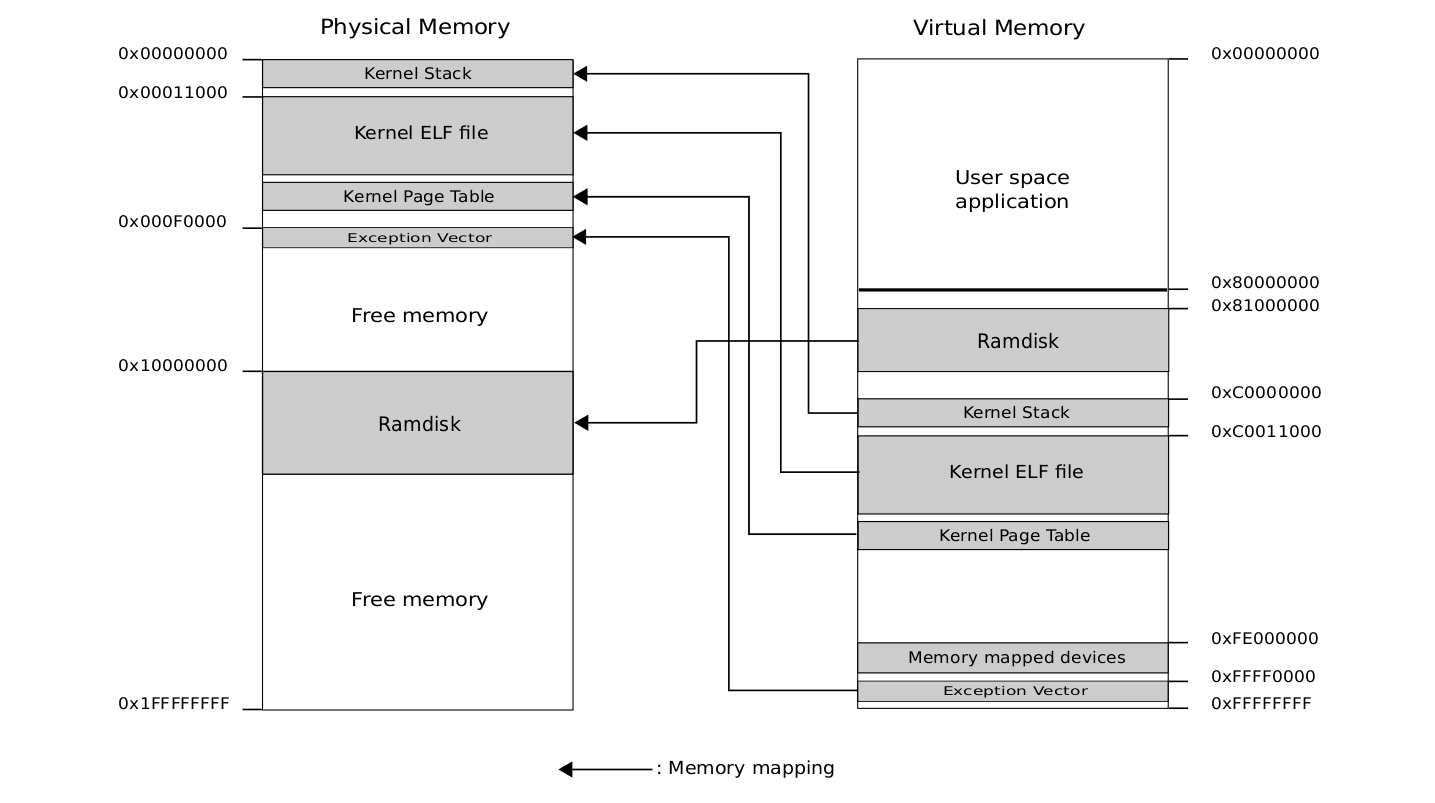
\includegraphics[width=\linewidth]{figures/memory_layout.png}
  \caption{Barrelfish memory layout for ARMv7 on GEM5}
  \label{fig:memory_layout}
\end{figure}

Figure~\ref{fig:memory_layout} shows the memory layout of the
single-core ARMv7-a port of Barrelfish. We have a memory split at 2GB,
where everything upwards is only accessible in privileged mode and the
lower 2GB of memory is accessible for user space programs. The
position of the kernel in the virtual space is hard- coded. The L1
page table of the kernel address space is located right after the
kernel and aligned to 16KB. We map the whole available physical memory
into the kernel’s virtual address space. The locations for the 64KB
kernel stack, the ramdisk aswell as the section for memory mapped
devices are hardcoded.  Overall the memory layout is very static and
turned out to be problematic with regard to multicore support, which
will be explained in section 4.2.


We still implement a memory split the same way we did in the
single-core port. The only real difference is that the kernel image
can now be loaded anywhere in memory instead of only at a fixed
location. The kernel stack and page tables are statically allocated
and part of the kernel image. Since the kernel is not statically
linked to a fixed address in high memory anymore, we have to relocate
the kernel image during boot up. We do this by adding our memory
offset constant (2GB) to the current kernel location to make sure the
kernel is in high memory after the relocation. The program counter and
stack pointer need to be relocated as well and we do this again by
just adding the memory offset constant to their current values. After
these relocations we can reset the 1:1 mapping of the physical memory
and only map in the high memory aliased regions to finally get our
desired memory layout. To simplify global shared data between kernels
at boot up, i.e. before the message passing has been set up, we
reserved the first MB of physical memory for this purpose.


%%%%%%%%%%%%%%%%%%%%%%%%%%%%%%%%%%%%%%%%%%%%%%%%%%%%%%%%%%%%%%%%%%%%%%%%
\bibliographystyle{abbrv}
\bibliography{defs,barrelfish}

\end{document}

\end{document}
